%% Bemærk:
%%          Resten af rapporten følger en stil hvor indledninger skrives
%%          med \sffamlily-typen. Denne stil bør også følges her.
%%
{\sffamily
I denne sektion vil vi afprøve den udvidede metode for at se, om den
virker efter hensigten på testbilleder og hvordan den virker i praksis
på udvalgte malerier.
}
\subsection{Afprøvning på testbilleder}
Vi afprøver metoden på 4 testbilleder. Billedet \ref{hus_virker} er et hus,
hvor snittet og massemidtpunktet næsten ligger oven i hinanden. 

\begin{figure}[h!!]
	\begin{center}
		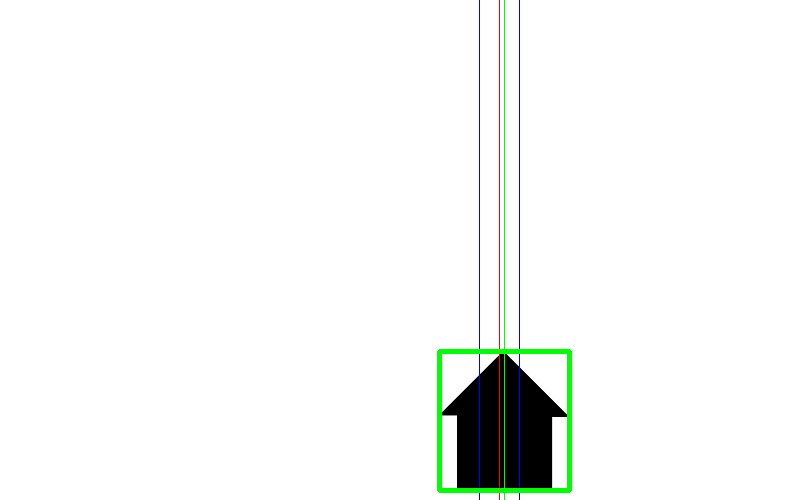
\includegraphics[angle=0,width=0.9\textwidth]{afsnit/afprovning/billeder/udvidet_losning/udvidet_hus1_test.png}
	\end{center}
	\caption[]{Et hus, der er symetrisk og har massemidtpunkt i spisen
	af taget. Massemidtpunktet er inde for margin, så huset bliver
	udvalgt til at ligge i snittet.}
	\label{hus_virker}
\end{figure}

I det andet billede, \ref{hus_virker_ikke}, er huset forskuppet, så massemidtpunktet ligger lige uden for margin, og derved skulle det ikke blive tage
med af metoden. 

\begin{figure}[h!!]
	\begin{center}
		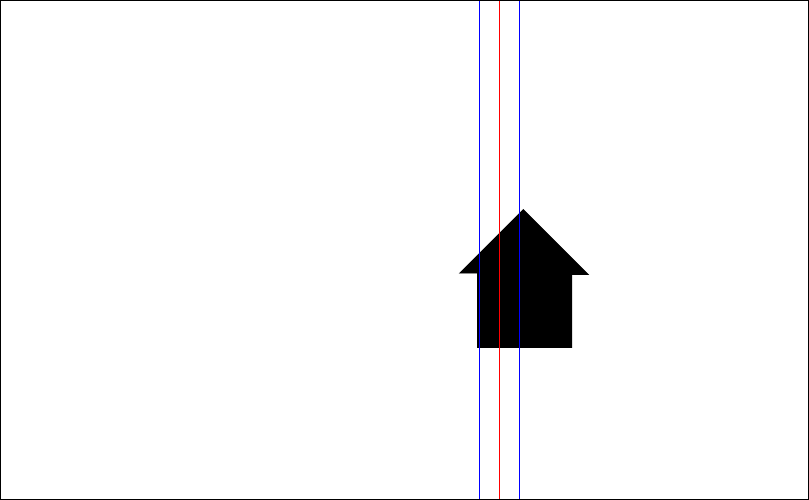
\includegraphics[width=0.9\textwidth,angle=0]{afsnit/afprovning/billeder/udvidet_losning/udvidet_hus2_test.png}
	\end{center}
	\caption[]{Hus, hvor massemidtpunktet er flyttet få pixels uden for margin. Den udvidede metode vælger ikke at tage huset med.}
	\label{hus_virker_ikke}
\end{figure}

Det tredje billedet, \ref{udvidet_blob_test}, har en region, som er
meget lille og derfor bliver sorteret fra. Den store region bliver taget
med, da dens massemidtpunkt ligger inden for margin. 

\begin{figure}[h!!]
	\begin{center}
		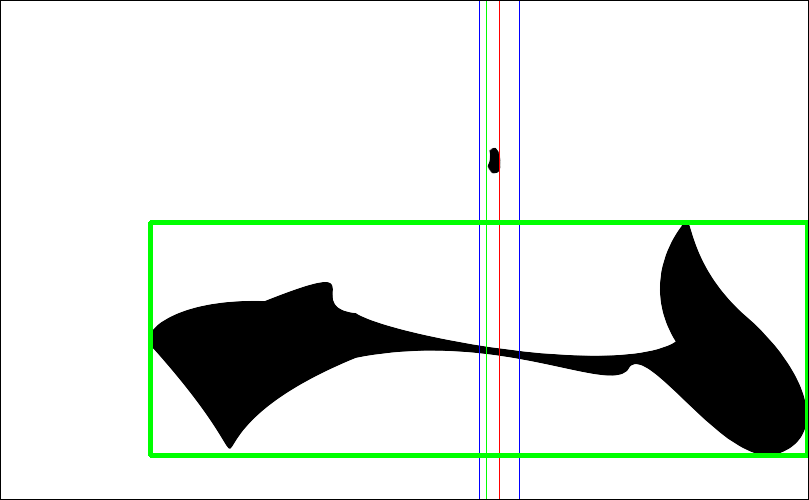
\includegraphics[width=0.9\textwidth,angle=0]{afsnit/afprovning/billeder/udvidet_losning/udvidet_blob2_test.png}
	\end{center}
	\caption[]{To regioner, hvor den nederste har et massemidtpunkt inden for margin.}
	\label{udvidet_blob_test}
\end{figure}

I det fjerde billede, \ref{bleksprutte_test} er der en region, som har
et massemidtpunkt inden for margin, men som har en skæv fordeling af pixels
i forhold til snittet og derfor bliver sorteret fra. Ud fra de fire
observationer, virker det som om, den udvidede metode virker efter
forventningerne.

\begin{figure}[h!!]
	\begin{center}
		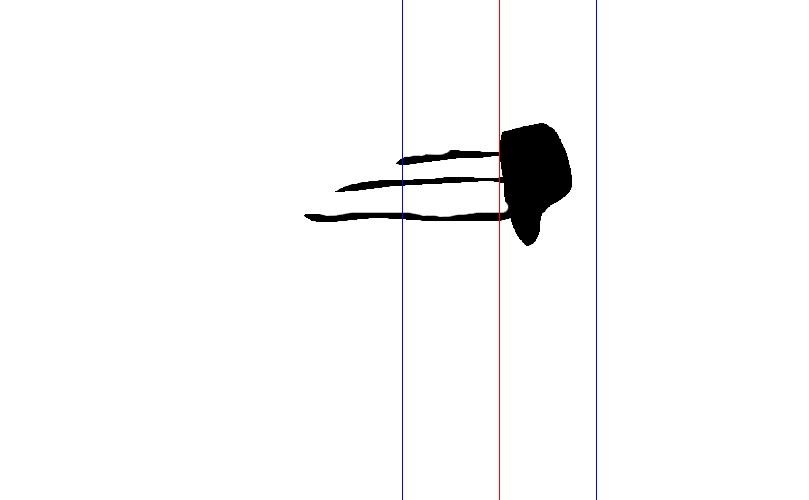
\includegraphics[width=0.9\textwidth,angle=0]{afsnit/afprovning/billeder/udvidet_losning/udvidet_bleksprutte_test.png}
	\end{center}
	\caption[]{Margin er sat meget op, så man kan se, at regionen har et massemidtpunkt inden for margin, men da størstedelen af regionens pixels er på højre side, vælges den fra.}
	\label{bleksprutte_test}
\end{figure}

Som man kan se af testbillederne, vælger den udvidedede løsning vidt
forskellige regioner til at ligge i snittet. 
\clearpage


\subsection{Afprøvning på malerier}
Afprøvningen af den udvidede metode på malerier fra vores database
foregår på samme måde som afprøvningen af den naive.

\begin{figure}[h!!]
	\begin{center}
		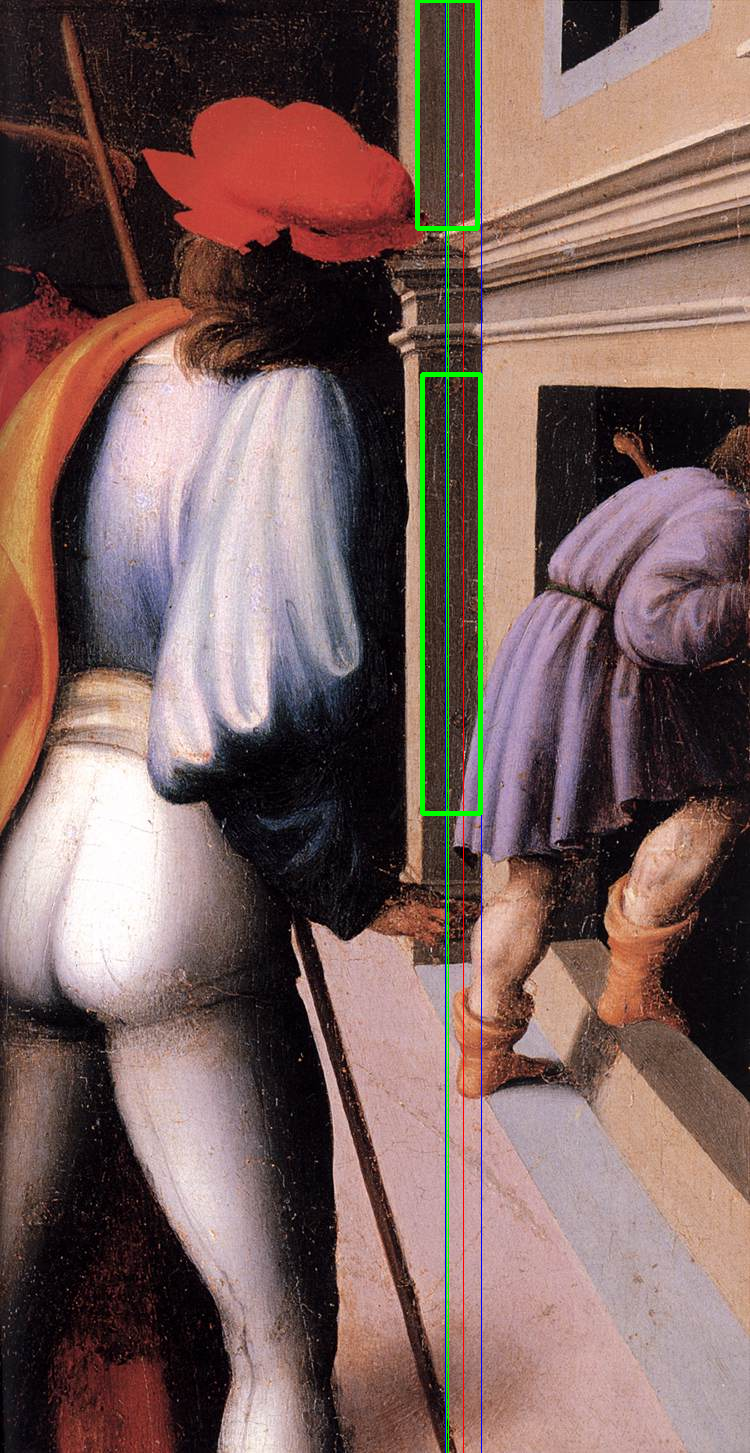
\includegraphics[width=0.85\textwidth,angle=0]{afsnit/afprovning/billeder/udvidet_losning/udvidet_kfarver_sdetaljer.png}
	\end{center}
	\caption[]{To ud af de seks regioner er godtager som liggende i det gyldne snit af den udvidede metode.}
	\label{udvidet_virker1}
\end{figure}

\begin{figure}[h!!]
	\begin{center}
		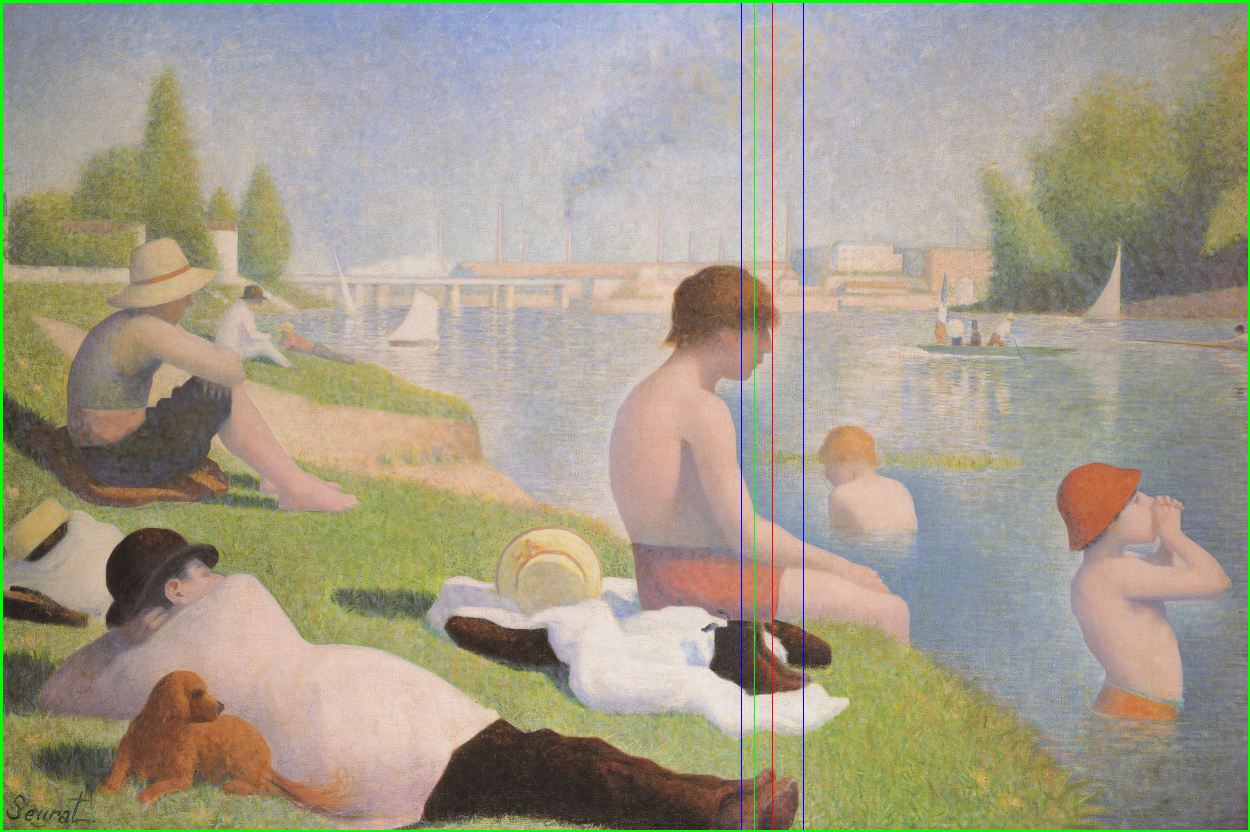
\includegraphics[width=0.9\textwidth,angle=0]{afsnit/afprovning/billeder/udvidet_losning/udvidet_dreng.png}
	\end{center}
	\caption[]{Baggrunden er den eneste region som bliver godtaget, da den har et massemidtpunkt, som ligger inden for marginen. Bemærk den grønne kant rundt om hele billedet.}
	\label{udvidet_virker2}
\end{figure}

\begin{figure}[!h]
    \centering
    	\subfloat[Udvidet metode.]{
        	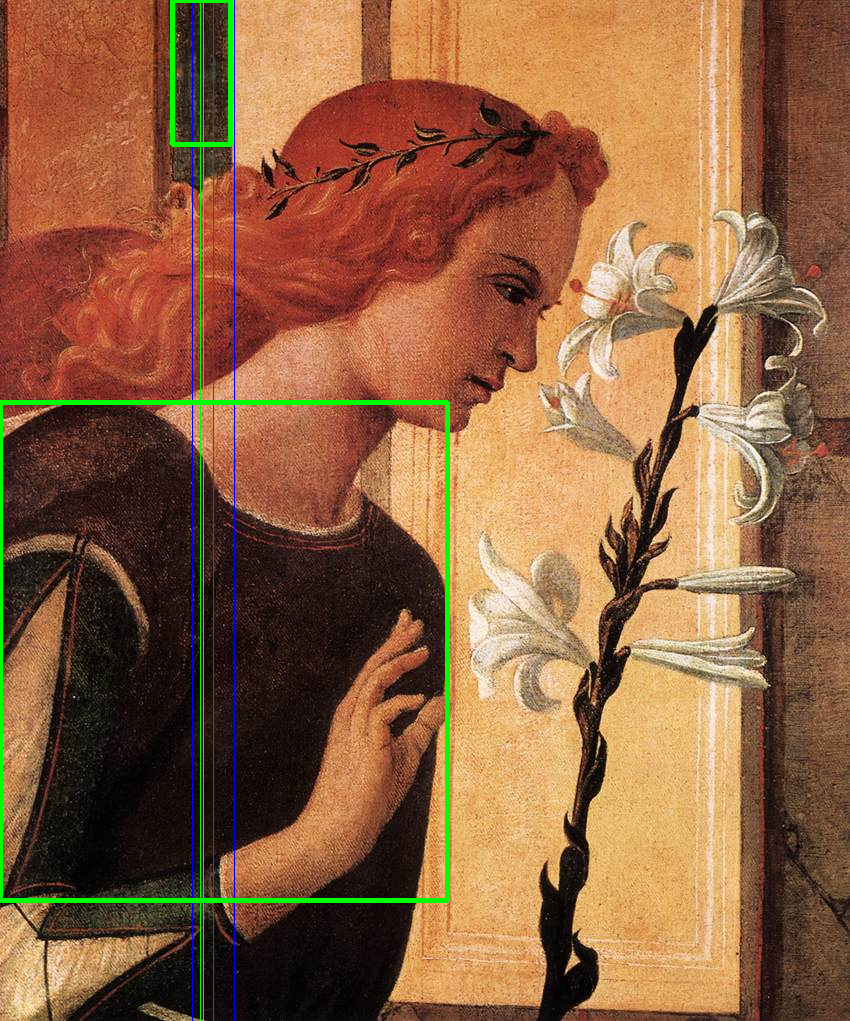
\includegraphics[angle=0,width=0.45\textwidth]{afsnit/afprovning/billeder/udvidet_losning/udvidet_pige.png}
        	\label{udvidet_pige}}\hspace{1em}
    	\subfloat[naiv metode.]{
        	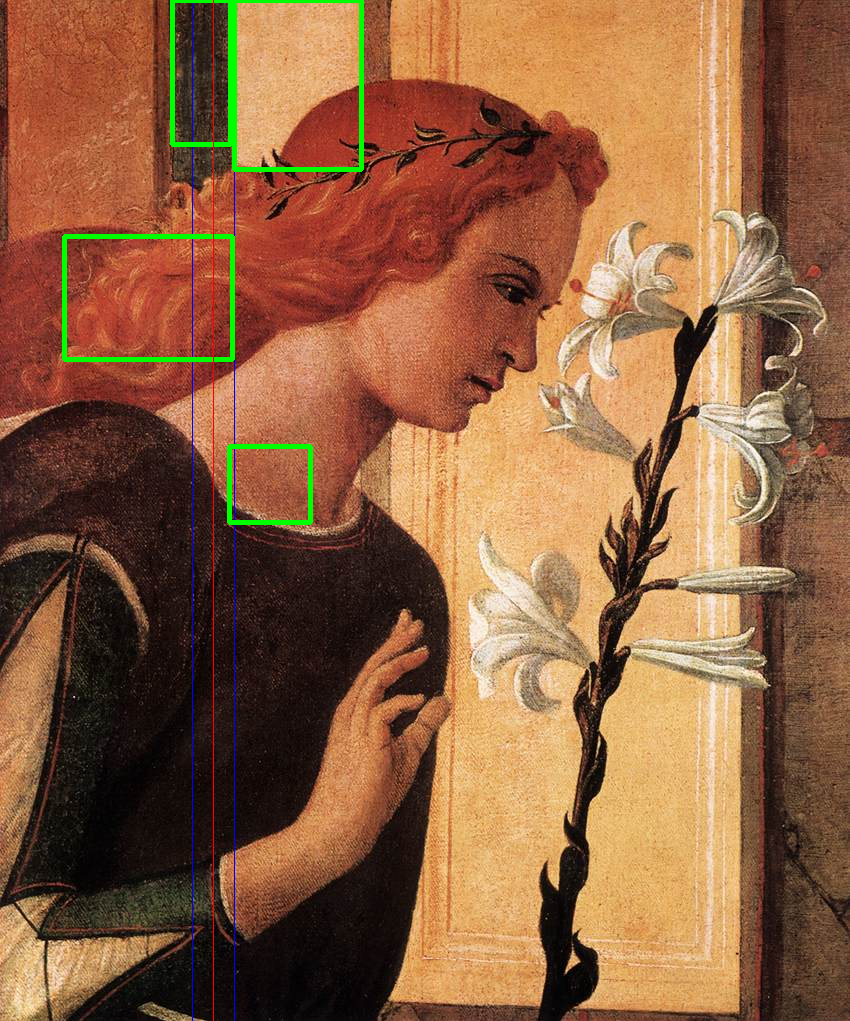
\includegraphics[angle=0,width=0.45\textwidth]{afsnit/afprovning/billeder/udvidet_losning/naiv_pige.png}
        	\label{naiv_pige}}\hspace{1em}        	    			
        \caption[]{Et maleri, hvor resultatet for den udvidede og den naive metode er vist. Der bliver fundet forskellige regioner for hver af metode. Navn: Angel Announcing. År ca. 1500. Af: Bellini, Giovanni.}
     \label{udvidet_virker3}
\end{figure}

\begin{figure}[h!!]
	\begin{center}
		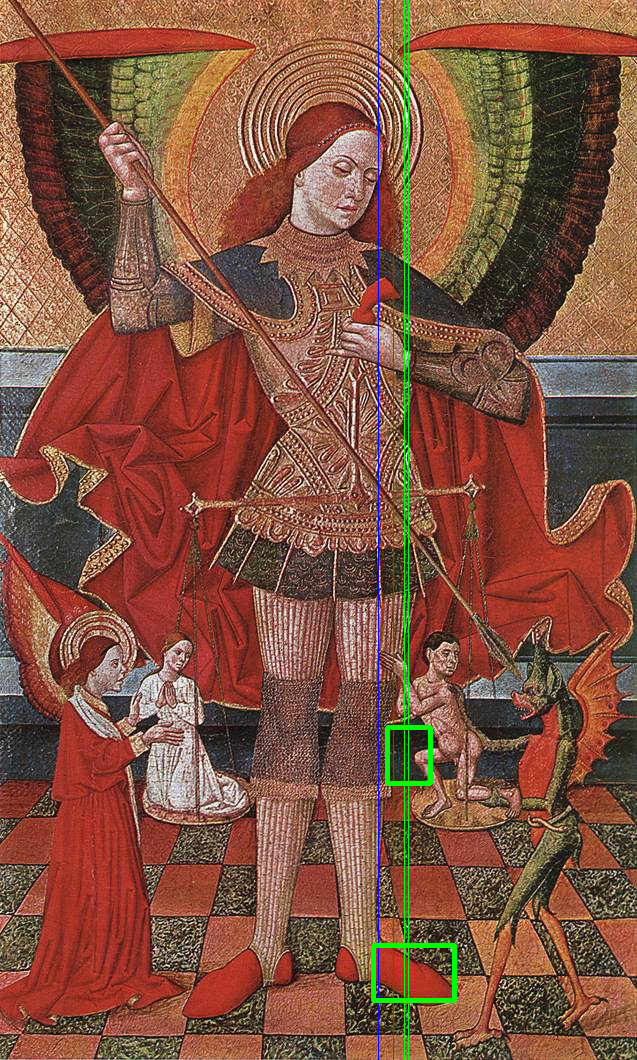
\includegraphics[width=0.9\textwidth,angle=0]{afsnit/afprovning/billeder/udvidet_losning/udvidet_kfarver_kdetaljer.png}
	\end{center}
	\caption[]{En sko og en flise bliver taget med at den udvidede metode.}
	\label{udvidet_virker_ikke1}
\end{figure}

\begin{figure}[h!!]
	\begin{center}
		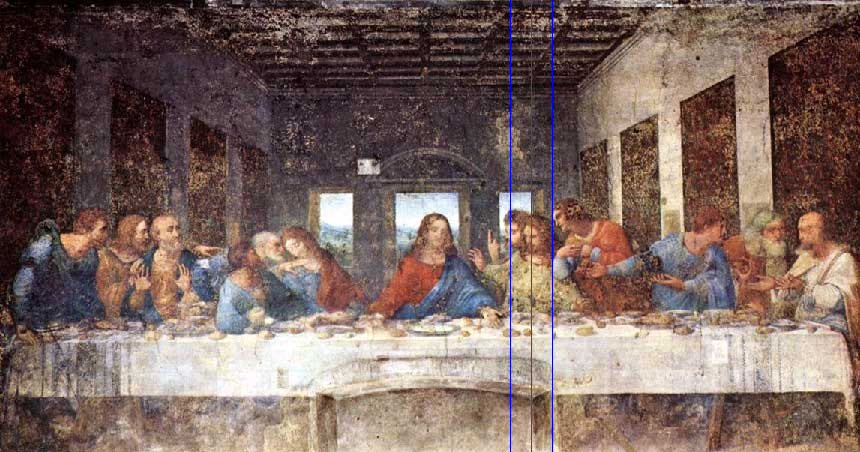
\includegraphics[width=0.9\textwidth,angle=0]{afsnit/afprovning/billeder/udvidet_losning/udvidet_mfarver_mdetaljer.png}
	\end{center}
	\caption[]{Den udvidede metode sorterer alle regioner væk.}
	\label{udvidet_virker_ikke2}
\end{figure}

\begin{figure}[h!!]
	\begin{center}
		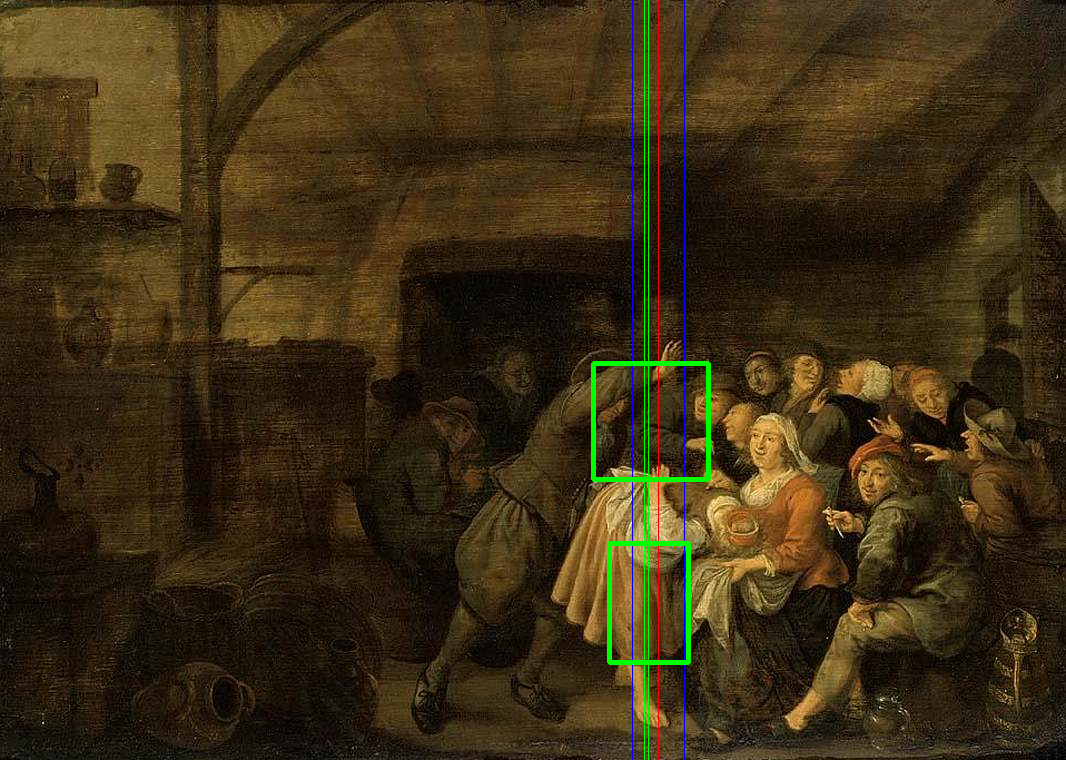
\includegraphics[width=0.9\textwidth,angle=0]{afsnit/afprovning/billeder/udvidet_losning/udvidet_sfarver_mdetaljer.png}
	\end{center}
	\caption[]{To regioner, som ikke repræsenterer noget i billedet, bliver fundet.}
	\label{udvidet_virker_ikke3}
\end{figure}


Ud fra tabellerne \ref{udvidet_good} og \ref{udvidet_bad}, hvor de
interressante og falske positiver er opstillet --- som i den naive
afprøvning --- kan det ses, at der blive fundet 7 interessante regioner og 5
falske positiver. Det vil sige 40 \% flere interessante regioner en falske
positiver.

\begin{table}[H]
    \centering
    \begin{tabular}{|c|l|l|l|}
	\hline
           				& Kraftige farver & Medium farver & Svage farver \\\hline
		Mange detaljer	& 1 & 0 & 1 \\\hline
        Medium detaljer & 0 & 1 & 0 \\\hline
        Få detaljer     & 0 & 0 & 4 \\\hline
    \end{tabular}
    \caption[]{Tabel over antal interessante regioner i det gyldne snit 0 i ni test malerier.}
    \label{udvidet_good}
\end{table}

\begin{table}[H]
    \centering
    \begin{tabular}{|c|l|l|l|}
		\hline
            & Kraftige farver & Medium farver & Svage farver \\\hline
		Mange detaljer	& 0 & 2 & 1 \\\hline
        Medium detaljer  & 0 & 3 & 0 \\\hline
        Få detaljer     & 2 & 3 & 0 \\\hline
    \end{tabular}
    \caption[]{Tabel over antal falske positiver i det gyldne snit 0 i ni test malerier.}
    \label{udvidet_bad}
\end{table}
\clearpage

\subsection{Konklusion}
Den udvidede metode virker som vi havde planlagt på de ensfarvede
regioner i testbillederne I praksis er den udvidede metode merer
effektiv end den naive: Som man kan se i figur \ref{udvidet_virker3} finder
den $20 \%$ flerer interessante regioner end falske positiver, end den
naive metode gør. Selv om den udvidede stadig kun finder $40\%$ flere
interessante regioner en falske positiver, er det ikke helt dårligt, i
betratning af, at vores regiondetektor ikke virker optimalt. Alt i alt
er det alså en god løsning.
